\Titular% 
{Donnie Darko: ciencia para estadounidenses?}%
{Emilia Prado Senlle}%
{divulgacion}%
{Breve disertación sobre a ciencia no filme \textit{Donnie Darko}.}%

\begin{refsection}
\begin{multicols}{2}


Existen moitas películas que tratan de incorporar a física nas súas tramas. O
exemplo máis notable é, probablemente, \textit{Interstellar}, coas súas viaxes
polo tempo e distintas realidades. Ademais, algo que adoitan compartir estes
filmes é a súa constante presenza en vídeos con títulos coma: <<\textit{10
películas que che farán explotar a túa mente!!!!}>> Que se viaxes no tempo, se
universos paralelos… Un lío. Claro que a confusión e a intelixencia non son
sinónimos, e o público xeral non tende a ser un bo crítico da rigurosidade
científica. Polo tanto, ao veren estes filmes que tanto xogan co espectador, a
pregunta real debería ser: é confuso porque é intelixente, ou simplemente
porque é estúpido?\\

\begin{centering}
    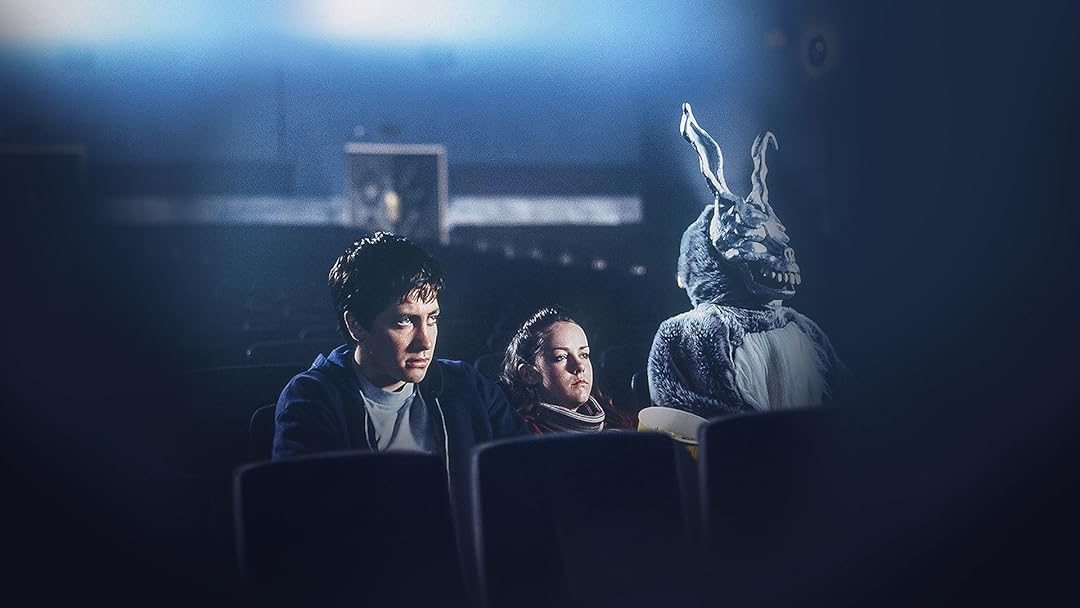
\includegraphics[width=1\linewidth]{revistas/002/imaxes/DONNIE-DARKO.jpg}
    \captionof{figure}{Fotograma, Donnie e Frank. \cite{donnie_darko}}
\end{centering}

Cando buscas Donnie Darko na Internet, a maior parte dos resultados van ser
unha versión de: <<\textit{final de \textbf{Donnie Darko} explicado con
\textbf{CIENCIA}!!!!}>>. Trátase dunha película comunmente coñecida polo seu
final confuso e a súa enrevesada cronoloxía. Foi dirixida por Richard Kelly e
rematou sendo considerada unha película de culto estadounidense tralo seu seu
lanzamento en 2001 e, máis tarde, en 2004, de \textit{Donnie Darko: The
Director’s Cut}, significativamente máis extensa ca a orixinal. A trama segue a
Donnie Darko, un adolescente que sofre de importantes problemas psicolóxicos e
comeza a alucinar cun coello xigante chamado Frank. Este coello salva a súa
vida dun accidente e avísao da inminente chegada do fin do mundo. A partir de
entón, Donnie vese obrigado a cumprir coas ordes de Frank, o que produce unha
serie de actos violentos ata o final, no que casualmente viaxa no tempo para
salvar o seu mundo da destrución.

A explicación máis común en vídeos de YouTube adoita ser unha: Donnie, ao
sobrevivir ao incidente, entrou nun universo paralelo que colapsará en pouco
tempo. Antes que iso poida ocorrer, viaxa a través do tempo ata o seu universo
de orixe, morre, e salva os seus amigos da apocalipse. Soa un pouco estúpido de
primeiras, mais o certo é que, se indagamos un pouco, podemos dar nas bases do
filme con nomes do mundo da física.

\subsection*{\textit{Donnie Darko} explicado con ciencia!}

Un concepto en que esta obra insiste moito é na de destino e determinismo, que
se presenta visualmente na forma dunha masa que se extende dende o peito de
cada ser ata o lugar onde vai estar no futuro; e aínda que semella estraño,
este é un concepto físico existente, aínda que algo reinterpretado. Os físicos
David Deutsch e Michael Lockwood explican que a vida forma unha especie de
``verme’' de 4 dimensións, cunha cola que representa a orixe da vida, e unha
cabeza na que se atopa a morte \cite{deutsch.m_1994}. Así, un obxecto como
o vemos no presente non é máis que a intersección nun espazo tridimensional
entre este e o seu ``verme'’.  Por suposto, a película céntrase máis no aspecto
filosófico desta cuestión; se podemos ver o futuro, significa que é inevitable?
Existe o destino? Está xa decidido que vou ser un fracasado? O cal é unha
pregunta moi interesante, e moi explorada dende tempos do determinismo
mecanicista do Renacemento ata a actualidade. Con todo, esta cuestión
científica e filosófica vese rapidamente destruída polo propio guión. Donnie,
en resposta ás dúbidas filosóficas do seu profesor de ciencias, di: <<non [está
decidido] se quedas na Canle de Deus>>\cite{donnie_darko}.
Así, fácil. Deus.\\

Podería opinarse que este intento por explicar o físico mediante o místico, ou
de incluír a Deus dunha forma tan repentina e fóra de lugar no argumento,
pódese ignorar un pouco ao ter en conta que o filme supón, en grande medida,
unha crítica á mentalidade cerrada e tradicionalmente relixiosa dos suburbios
americanos. Ademais, ao recurrir á versión de corte do director da película,
ofrécesenos unha explicación sobre o universo de Donnie moito máis completa ao
incluír extractos do libro de Roberta Sparrow, outra personaxe da película.
Este leva o nome de \textit{A Filosofía das Viaxes no Tempo}, e fala sobre a
formación de Universos Tanxentes extremadamente inestables a partir de
incidentes no Universo Primario. Iso explicaría todo o tema da fin do mundo,
pero… realmente ten sentido?

É obvio que os universos paralelos ou múltiples non son un tema inexplorado
pola física moderna. Por exemplo, para explicar a `superposición’ das
partículas subatómicas en múltiples estados instantáneos, Hugh Everett refírese
ao que posteriormente se bautizou como a \textit{Interpretación de Mundos
Múltiples}. Esta describe que cada un dos estados nos que atopamos unha
partícula ocorren simultaneamente, só que en distintas ramas do universo e cada
vez que tratamos de observala, o universo divídese en distintas realidades
paralelas \cite{gribbin2004historia}. É claro que esta non é unha tese demasiado
consolidada no mundo científico, xa que non hai forma de demostrala
experimentalmente. Pero existe e é obvio que Donnie Darko bebe destas ideas;
nun universo, Donnie está vivo, e noutro, morto.

Pois, entón, estas realidades non deberían interactuar de ningunha forma, non
si? Como pode ser que Donnie volva ao seu universo orixinal ao final da
película? Ou que Frank, que é en realidade o amigo morto de Donnie, volva atrás
no tempo para avisar da fin do mundo? Pois ben, a película realmente non o
explica. O libro de Roberta Sparrow menciona as viaxes no tempo, mais cunha
explicación vaga e demasiado mística para ser científica, <<\textit{A Auga e o
Metal son os elementos chave para as Viaxes no Tempo. A Auga é o elemento
barreira para a construción de Portais de Tempo que conectan Universos no
Vórtice Tanxente}>> \cite{donnie_darko}.\\

Con todo, na física, existe quen tratou estes problemas. Por exemplo, Kurt
Gödel e a súa métrica de Gödel, coa que pretendeu solucionar as ecuacións de
campo de Einstein. Esta presenta a existencia de cadeas causais pechadas, nas
que o evento orixinal se causa a si mesmo \cite{nunez.r_2021}. Claro que esta é unha
teoría que se cuestiona profundamente como verdadeira (véxase o paradoxo do
avó). Aínda así, é algo interesante de explorar; a pesar de que a película nin
tan sequera trate de facelo, máis aló de referirse a unha viaxe no tempo
inexplicable, a partir dun buraco no espazo-tempo inexplicable, e cunhas
consecuencias… dubidosas. É obvio que así vai quedar un final, como mínimo,
confuso.

\subsection*{Cine e... ciencia?}

Por suposto, isto non significa que unha película deba ofrecer unha explicación
pormenorizada, argumentada e cun sentido científico riguroso. Ao final, é
ficción, e perdería un pouco a graza se houbese que incluír unha bibliografía
citada en Harvard ao final dos créditos. E o certo é que a trama ten as súas
bases, ata certo punto. Con todo, resulta dubidoso cando unha obra trata de
parecer profundamente complexa e intelixente cando non é máis que uns cantos
conceptos físicos empregados ao servizo do guión; e cando a conversación máis
científica que podemos escoitar nela é a explicación dun profesor de instituto
sobre o que son os vectores no espazo. Ao final do día, tampouco se pode culpar
disto a un filme tan claramente feito para o público estadounidense xeral.

\nocite{deutsch.m_1994}
\nocite{donnie_darko}
\nocite{gribbin.j_2020}
\nocite{nunez.r_2021}
\nocite{wisecrack_2019}

\printbibliography

\end{multicols}
\end{refsection}
